\DiaryEntry{The Greatest-Integer (Floor) Function}{2021-01-25}{Number Theory}

This is based on \cite{Burton2011}, Section 6.3.

For any real number $x$, we denote by $\lfloor x \rfloor$ the largest integer less than or equal $x$. In other words, $\lfloor x \rfloor$ is the unique integer satisfying $x-1 < \lfloor x \rfloor \leq x$.

In case of positive numbers, everything is quite easy; e.g. we have $\lfloor 4 \rfloor = 4, \lfloor 4.1 \rfloor = 4, \lfloor \pi \rfloor = 3$. In case of negative numbers, we need to consider $-4 < -3$ and therefore we have $\lfloor -4 \rfloor = -4$, but (maybe intuitively) $\lfloor -4.1 \rfloor = -5$.

The equality $\lfloor x \rfloor = x$ holds only when $x$ is an integer and we can write any real number $x$ as

\bee
x = \lfloor x \rfloor + \theta
\eee

with $0 \leq \theta < 1$.

The following Figure shows a plot of the floor function.

\begin{figure}[H]
    \centering
    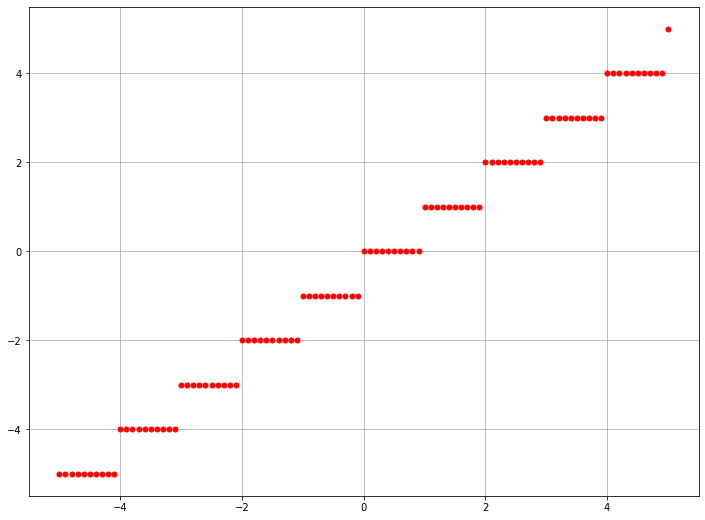
\includegraphics[scale=0.5]{images/floor_function.png}
\end{figure}


An interesting observation regarding the floor function is

\bee
\lfloor a + b \rfloor \geq \lfloor a \rfloor + \lfloor b \rfloor
\eee

We need to consider two cases: In the first case, $a + b = \lfloor a + b \rfloor + \theta$ with $0 \leq \theta < 1$. Then $\lfloor a+b \rfloor = \lfloor a \rfloor + \lfloor b \rfloor$. This is the case for e.g. $\lfloor 0.3 + 0.5 \rfloor = 0 = \lfloor 0.3 \rfloor + \lfloor 0.5 \rfloor$. In the second case, the sum $a + b$ yields a larger result, we have $a + b = \lfloor a + b\rfloor + 1 + \theta$ with $0 \leq \theta < 1$. Then $\lfloor a + b \rfloor > \lfloor a \rfloor + \lfloor b \rfloor$. This is the case of e.g. $\lfloor 0.7 + 0.8 \rfloor = 1 > \lfloor 0.7 \rfloor + \lfloor 0.8 \rfloor = 0$.

Combining both cases yields the above inequality.

In a similar spirit, we have for positivie $a, b$,

\bee
\lfloor ab \rfloor \geq \lfloor x \rfloor \lfloor y \rfloor
\eee

The floor function appears also in a number-theoretic context as follows: We want to know how often a particular prime $p$ appears in $n!$. E.g. $p = 3, n = 10$, then

\begin{align*}
    10! &= 1 \cdot 2 \cdot 3 \cdot 4 \cdot 5 \cdot 6 \cdot 7 \cdot 8 \cdot 9 \cdot 10 \\
    &= 1 \cdot 2 \cdot 3 \cdot 2^2 \cdot 5 \cdot 2 \cdot 3 \cdot 7 \cdot 2^3 \cdot 3^2 \cdot 2 \cdot 5 \\
    &= 2^8 \cdot 3^4 \cdot 5^2 \cdot 7
\end{align*}

so $3$ is contained $4$ times in $10!$. The following theorem provides a way for calculating this number.

\begin{theorem}
    If $n$ is a positive integer and $p$ a prime, then the exponent of the highest power of $p$ that divides $n$ is

    \bee
        \sum_{k=1}^\infty \left\lfloor \frac{n}{p^k} \right\rfloor
    \eee

    where the series is finite, as $\lfloor n/p^k \rfloor = 0$ for $p^k > n$.
\end{theorem}

In the example of $n=10, p=3$ from before, we have

\bee
\sum_{k=1}^\infty \left\lfloor \frac{n}{p^k} \right\rfloor = \left\lfloor\frac{10}{3}\right\rfloor + \left\lfloor\frac{10}{9}\right\rfloor = 3 + 1 = 4
\eee

From the first $n$ positive integers, those divisible by $p$ are $p, 2p, 3p, tp$ where $t$ is the largest integers such that $tp \leq n$; i.e. $t = \lfloor n/p \rfloor$. Therefore, we have $\lfloor n/p \rfloor$ multiples of $p$ occuring in the product that defines $n!$, namely,

\bee
p, 2p, \ldots, \left\lfloor \frac{n}{p} \right\rfloor p
\eee

In our running example, these are the numbers $3, 6, 9$. There are $\lfloor 10 / 3 \rfloor = 3$ of them.

We continue with the number of integers from $1, 2, \ldots, n$ which are divisible by $p^2$. These are the following $\left\lfloor \frac{n}{p^2} \right\rfloor$ numbers

\bee
p^2, 2p^2, \ldots, \left\lfloor \frac{n}{p^2} \right\rfloor p^2
\eee

In our running example, this is the number $9$; i.e. $\lfloor 10 / 9 \rfloor = 1$ number.

We can continue with higher exponents of $p$; however, we have fewer and fewer terms with increasing exponents. Eventual $p^k$ will be so large, that $n > p^k$ and we won't have any further terms. Summing all terms up, we arrive at the number of times $p$ divides $n$ by

\bee
\sum_{k=1}^\infty \left\lfloor \frac{n}{p^k} \right\rfloor \qed
\eee

Note that we do \emph{not} overcount factors; i.e. $3$ divides $3, 6, 9$ and $3^2 = 9$ divides $9$. So, \emph{in total}, $3$ divides $10!$ $4$ times.

We can use the result for a different representation of the factorial; namely

\bee
n! = \prod_p p^{\sum_{k=1}^\infty \left\lfloor \frac{n}{p^k} \right\rfloor}
\eee

\paragraph{Example.} We can use above theorem to calculate the number of zeros of $11!$. This is given by the exponent of $10$ contained in $11!$. Since $10$ is not a prime, we need to use a little trick: We determine how often $2$ is a factor of $10!$ and then how many times $5$ is a factor of $10!$. The smaller of the two determines how often $10$ is contained in $11!$.

For $2$ we have

\bee
n_2 = \left\lfloor \frac{11}{2} \right\rfloor + \left\lfloor \frac{11}{2^2} \right\rfloor + \left\lfloor \frac{11}{2^3} \right\rfloor = 5 + 2 + 1 = 8
\eee

and for $5$ we have

\bee
n_5 = \left\lfloor \frac{11}{5} \right\rfloor = 2
\eee

The smaller of the two numbers is $n_5 = 2$; therefore $10^2 = 100$ is the largest exponent of $10$ which divides $11$ and therefore $11!$ has two zeros. We have $11! = 39916800$ which shows the correctness of the result.

We know from previous entries that for positive integers $r,n$ with $1 \leq r < n$, the binomial coefficent

\bee
{n \choose k} = \frac{n!}{r!(n.r)!}
\eee

is an integer. From this we deduce that for a positive integer $n$, the product of any $r$ consecutive integers is divisible by $r!$. The product is given as

\bee
n(n-1)(n-2) \cdots (n - r + 1)
\eee

We can write this as

\bee
n(n-1)(n-2) \cdots (n - r + 1) = \frac{n!}{(n-r)!} = \frac{n!}{r!(n-r)!}r! = {n \choose r} r!
\eee

Since the binomial coefficient is an integer, $n(n-1)(n-2) \cdots (n - r + 1) / r!$ is also an integer. \qed

We finally have the following theorem.

\begin{theorem}
    Let $f$ and $F$ be number-theoretic functions with

    \bee
        F(n) = \sum_{d | n} f(d)
    \eee

    For any positive integer $N$, we have

    \begin{equation}
        \sum_{n=1}^N F(n) = \sum_{k=1}^N f(k) \left\lfloor \frac{N}{k} \right\rfloor
    \end{equation}

\end{theorem}

Our number theoretic functions $\tau(n)$ and $\sigma(n)$ can be expressed as (see entriy \ref{2021-01-18:entry})

\bee
\tau(n) = \sum_{d | n} 1, \qquad \sigma(n) = \sum_{d | n} d
\eee

and we therefore can apply the previous theorem for the sums

\bee
\sum_{n=1}^N \tau(n) = \sum_{k=1}^N \left\lfloor \frac{N}{k} \right\rfloor, \qquad \sum_{n=1}^N \sigma(n) = \sum_{k=1}^N k \left\lfloor \frac{N}{k} \right\rfloor
\eee

As an example, consider $N = 6$. We have $\sum_{k=1}^6 \tau(n) = 14$ and $\sum_{k=1}^6 \sigma(n) = 33$. Using the sums, we obtain

\bee
\sum_{n=1}^N \tau(n) = \sum_{k=1}^6 \left\lfloor \frac{6}{k} \right\rfloor = \lfloor 6 \rfloor + \lfloor 3 \rfloor + \lfloor 2 \rfloor + \lfloor 3/2 \rfloor + \lfloor 6/5 \rfloor + \lfloor 1 \rfloor = 14
\eee

and

\bee
\sum_{n=1}^N \sigma(n) = \sum_{k=1}^6 k \left\lfloor \frac{6}{k} \right\rfloor = 1 \lfloor 6 \rfloor + 2 \lfloor 3 \rfloor + 3 \lfloor 2 \rfloor + 4 \lfloor 3/2 \rfloor + 5 \lfloor 6/5 \rfloor + 6 \lfloor 1 \rfloor = 33.
\eee



%%% Local Variables:
%%% mode: latex
%%% TeX-master: "journal"
%%% End:
